%% LyX 2.1.4 created this file.  For more info, see http://www.lyx.org/.
%% Do not edit unless you really know what you are doing.
\documentclass[english]{article}
\usepackage[LGR,T1]{fontenc}
\usepackage[latin9]{inputenc}
\usepackage{geometry}
\geometry{verbose,tmargin=1.5cm,bmargin=1.5cm,lmargin=1.5cm,rmargin=1.5cm}
\usepackage{amsmath}
\usepackage{amsthm}
\usepackage{graphicx}
\usepackage{esint}

\makeatletter

%%%%%%%%%%%%%%%%%%%%%%%%%%%%%% LyX specific LaTeX commands.
\DeclareRobustCommand{\greektext}{%
  \fontencoding{LGR}\selectfont\def\encodingdefault{LGR}}
\DeclareRobustCommand{\textgreek}[1]{\leavevmode{\greektext #1}}
\DeclareFontEncoding{LGR}{}{}
\DeclareTextSymbol{\~}{LGR}{126}

%%%%%%%%%%%%%%%%%%%%%%%%%%%%%% Textclass specific LaTeX commands.
\numberwithin{equation}{section}
\numberwithin{figure}{section}

\makeatother

\usepackage{babel}
\begin{document}

\title{workshop - Anomaly Detection and Characterization in time series}


\author{Adi Berger - 301044657, Idan Attias, Gilad Rubin}

\maketitle

\section{Introduction}

Anomaly detection in time series is a challenging problem with numerous
potential applications. A comprehensive anomaly detection approach
not only should be able to detect and identify the emerging anomalies
but also to characterize the essence of these anomalie in a way that
is understandable to the end-user as well. Our goal is to create a
generic tool which according to a business KPI implements a comprehensive
anomaly detection and visualize the results for the end user. the
KPI is the attribute which the business wish to analzyze during time.
Thus, we sought to produce a generic tool which will work on every
data set that composed of events over time, with the given KPI attribute
and the features collected on that event.\\
Based on our data exploration process, we have discovered that many
anomalies are caused by some underlying process which affects only
a particular subset of the data. For example: if we look at the Request
Duration attribute over time splitted by the RoleInst attribute:\\
\\
 \includegraphics[scale=0.7,bb = 0 0 200 100, draft, type=eps]{role inst.png}\\
It is clear to see that the subset of data with attribue RoleInst
= RD000D3A002CF6 is a potential lead for the anomaly seen in the plot.
\\
In order to detect the underlying causes for the anomalies seen in
the data, we implemente a model which consists of two main steps:
we first use an anomaly detector on the whole dataset to identify
individual records with anomalous attribute values (the KPI attribute),
secondly, we detect and rank leads for the underlying causes for the
given anomolous records. We carry out this method by performing an
exhaustive search over many subsets of the data in order to find the
most probable common denominator for the anomalies. We wish to detect
any such subset of data which displays a significant increase in anomalous
activity as compared to the normal behavior of the system. We perform
significance testing to determine if any subset of the data is significantly
different than expected.\\
To evaluate the proposed method, we synthesized data and investigated
the results. 


\section{Model workflow}


\subsection{The workflow of our model is depicted below:\protect \\
\protect\includegraphics[scale=0.5,bb = 0 0 200 100, draft, type=eps]{diagram.png}\protect \\
In order to analyze a given dataset, each record in it must contain
a Timestamp, a KPI attribute (numeric value) and categorical attributes
related to that event.}


\subsection{With the abovementioned generic dataset, we aggregate the events
into a pre-defined time window, calculate the average of the KPI attribute
in each window and create a time series based on these values. }


\subsection{In order to choose the optimal time-window size, we implemented an
algorithm which searches through different time windows and other
parameters related to the outlier detection algorithm and used the
values which gave the highest f-score using a labeled synthesized
dataset. \protect \\
With the previously selected optimal parameters, we insert the time
series into an anomaly detection algorithm, based on STL decomposition
(See ......) and present the detected anomalies to the end-user, highlighted
in colors according to their severety. }


\subsection{Following the anomaly detection procedure, we treat each anomaly
seperately by taking all the combinations of attribute-values that
exist in the anomaly time window, limited to a combination of up to
3 attributes. for instance if the anomaly window contains the records:
\protect \\
\protect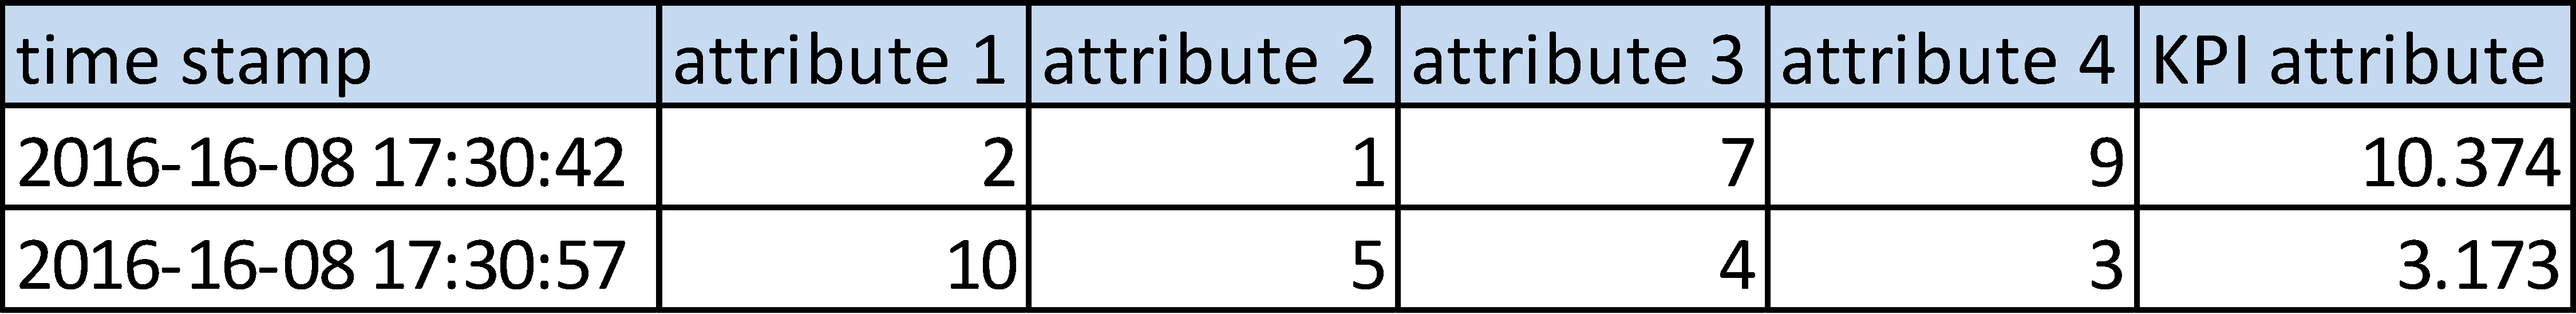
\includegraphics[scale=0.1,bb = 0 0 200 100, draft, type=eps]{demonstrate for workshop.emf}\protect \\
The following 1-tuple combinations can be: (attribute 1 = 2); (attribute
1 = 10); (attribute 2 = 1); (attribute 2 = 5) etc...\protect \\
With a combination of 2-tuples, we perform a cartesian product between
the distinct values of each feature, for example: (attribute 1 = 2,
attribute 2 = 1); (attribute 1 =2, attribute 2 = 5) etc...}


\subsection{Given a tuple a specific anomaly, we create a new data set by eliminating
the records containing this tuple from the original data set. then,
we aggregate the data set as explained before and run the same anomaly
detection on the filtered dataset. Our hypothesis is that if the algorithm
doesn't show an anomaly on the same point as the inspected anomaly
- we have a strong indication that this tuple may be an informative
lead for the anomaly. We have confirmed this hypothesis via our tests
(See .......). }


\subsection{From the algorithm results we get the anomalies and the predictive
values for each point on the time series. If on the new data set the
anomaly remains, significantly different from the expected value by
confidance level of 95\%. it means that this tuple wasn't the cause
for that anomaly. For the suspiciuos tuples (the ones that could cause
the anomaly) we use the results to measure 3 different scores that
supply informative data on those tuples:}


\subsubsection{New distance - at the anomaly point, the new distance from the expected
value in standard deviation (the lower it is the stronger indication
this tuple caused the anomaly)}


\subsubsection{Unique anomalies - how much anomalies found that didn't appear on
the former data set (which indicates ...)}


\subsubsection{Overall anomalies = 1- The percentage of common anomalies for both
data sets. which means, the percentage of anomalies this tuple removed
from the origin data set. that gives an indication if this tuple is
problematic, causing a lot of anomalies. (maybe false positive, maybe
allready known problem...). make it feasible to carry out a review
of all the historical events related to that context of the data}


\subsection{After having the scores for all the remainig tuples, we cluster them
according to scores New distane and Unique anomalies. After some experiments
we figuerd out that only the first score is not enough because if
the tuple records are a major portion of the data. the new time series
is not similar to the old one and the fact that there is no anomaly
on that point in the new time series can result from the fact that
a big number of records were removed. so using the second score is
to solve just that. From the clustered tuples we take the closest
cluster to the origin. beacuse the lower both scores are the greater
percentage the tuple explain the anomaly. We present to the end user
a list consist from all that tuples ordered by the third score overall
anomalies.}


\section{Data Preparation Process}

We chose to focus on the request duaration KPI. The data preprocessing
can be summarized in two steps:


\subsection{Select and Preprocess data}

We've noticed there is a lot of data available which contains information
about request duration, our chosen KPI. We picked the relevant files
and merge them to one csv file with all the information.\\
We filtered out columns that had full corelation to other column (where
the remain column explian the other) and columns that were very sparse
(more than 80\% missing values). We ended up with a large data set
(\textasciitilde{}700K rows), each row represents a request event
with request duration, time stamp and some more attributes. In this
created data set we replaced the nan values with Null value, gave
the correct type for each attribute: date time for timestamp, float
for request duration and categorical to the rest attributes. Furthermore,
the data was noncontinuous from the date: 2015-10-07 18:00. and due
to our on the continuity and seasonality of the data 


\subsection{Transform Data}

As explained in the above section. we divided the data according to
the time window received from the algorithm we ran on the synthetic
data (add algorithm explanation..), we calculated the average of the
KPI attribute in each window and create a new data set composed of
time series and the aggregated values


\section{Anomaly detection}


\subsection{Approaches:}

we implemented 3 different algorithms for anomaly detection...


\subsubsection{TSO}

.... blabla.r with the code


\subsubsection{Arima}


\subsubsection{STL}

we perform a seasonality adjustment using the STL decomposition method
and smoothing of the Trend element using Friedman's ``Super Smoother''.
We subtract the ``smoothed'' trend from our seasonally adjusted
time series and then we are left with a time series of residuals.


\subsection{comparison and which one we chose}

pros and cons/ trade offs of those approaches and which one we chose
to our model and why


\section{Anomaly characterization}


\subsection{Finding suspicious subsets}

we tried 3 different approaches, explained below. 


\subsubsection{New time series}


\subsubsection{P-Value}

For an anomaly we take all the combinations of values that exist in
the anomaly time window. for each such tuple we extracted distances
vector. distances vector represents the distance of all the request
duration (KPI attribute) of the selected subset events, from the average
of all the events excluding this subset, at each point this subset
had an event. meaning, how far the events of that subset are usually
from all the rest of the data. this vector is produced for all the
events that accured before the anomaly we wish to explore. for this
new vector of samples we fitted a distribution, and estimated according
to the recieved distribution the p-value of the distance at the anomaly
point. the distance at the anomaly point calculated as the distance
from the subset event request duration to the predicitive value received
from the STL algorithm. the p-value score gives strong indication
if this subset actually characterize the anomaly. because the lower
the value is the lower the probability for the given distance. which
means we can assume that this subset chracterize the anomaly and we
should take it under considuration for representing it to the end
user.\\
You can learn more about the implementation of this procedure in the
appendix


\subsubsection{Regression tree classifier}

For an anomaly, we take the predictive value received from the STL
algorithm (explained above). For each tuple that exist in the anomaly
time window, we calculated the distance in standard deviation (received
also by the algorithm) from the predictive value. We used the regression
tree algorithm for clustering those tuples according to that distance
and limiteded the tree depth to level 4. Regression tree do not require
the assumptions of statistical models and has the ability to automatically
bin massively categorical variables into a few categories. Hence,
variable selection \& reduction is done automaticly. We used those
properties and the fact that regression trees is relatively fast,
even with large data sets, for optimization. Instead of anlayze the
whole features values combinations, We looked only at the values combinations
created by the tree. when a combination is not only the nodes on a
path from root to a leaf. but also all the subgroups of this path
(from root to node). Because, those values explain in a good way the
distribution of the tuples around the anomaly. this approach improves
the efficiency of the model but lower the accuracy


\subsubsection{winning approach}

because the emphasis of our model is on characterize the anomalies
with high accuracy

relatively fasr, optimization for subsets selection.. easy to understand.
accuracy nore important because we emphasis on characterization we
decided to analyze all the subsets 


\subsection{Score subsets}


\subsection{Cluster subsets}


\subsection{Rank subsets}


\section{Synthetic Data Set}

The goal is to create a supervised data set for illustrating and testing
our model. We aimed to synthesize data which preserves our data properties
in terms of seasonality and trend. But, we didn't want to synthesize
a very simillar data set, because, our goal was to create a generic
method. So, the creation of points around that seasonality and trend,
didn't rely on the original data set events charasteristic (as their
standard deviation around the mean etc.). 


\subsection{creating data set}

First of all, to acheive the main properties about our data, we trimmed
the events with request duration value greater than $\pm$3 standard
deviations from the mean. In order to create seasonality and trend,
we calculated the average request duration per day and per hour. Furthermore
we calculated the ratio of the average request duration of an hour
and average request duration of a day, assuming that this ratio is
similiar for each hour and day (based on the seasonality we have seen
in our data). For each hour we created approximately 4000 (number
of events per hour on average) random time stamps, then attached to
it request duration values that were generated from normal distribution
with proper mean and standard deviation for this hour. We added to
this data frame another 4 columns which represents our attributes.
Each coulmn values were generated from different discrete distributions.
The choice of discrete distributions is owing to the fact that our
original features are categorical. 1 attribute was chosen from discrete
uniform distribution, 2 attributes from (different) binomial distributions
and another attribute from poisson distribution. 


\subsection{insert anomalies}

At this point we want to inject artificial anomalies in random time
stamps, and randomly choose how many features and which features to
be the cause of the anomaly. In addition, we generated randomly a
value which is the strength of the anomaly. That way, we will have
different kind of anomalies (global and seasonal). For each event
in the anomaly time range that contains the ``problematic'' features,
we increase the request duration- add to this value the multiplication
of the strengh of the anomaly with the standard deviation that was
calculated the previous stage. We recored the properties of each anomaly
so we can measure our result on the synthetic data. In the end, we
export our synthetic data frame to csv file. Illustration of the synthetic
data with anomalies:\\
\includegraphics[scale=0.7,bb = 0 0 200 100, draft, type=eps]{100_5-15.png}


\section{Appendix}


\subsection{p-value calculation}


\subsubsection{Fitting Distribution to data sample:}

\noindent Fitting distributions consists in finding a mathematical
function which represents in a good way a statistical variable. For
some observations of a quantitative character $x_{1},...,x_{n}$ we
wishes to test if those observations, being a sample of an unknown
population, belong from a population with a pdf (probability density
function) f(x,\textgreek{j}), where \textgreek{j} is a vector of parameters
to estimate from available data. \\
We can identify 3 steps in fitting distributions:
\begin{enumerate}
\item Model/function choice: hypothesize families of distributions; 
\item Estimate parameters;
\item Goodness of fit statistical tests.
\end{enumerate}

\subsubsection{Model choice:}

On the paper Probabilistic approaches to risk by Aswath Damodaran.
In Appendix 6.1 Aswath discusses the key characteristics of the most
common distributions and in Figure 6A.15 he provides us with a decision
tree diagram for choosing a distribution:\\
\\
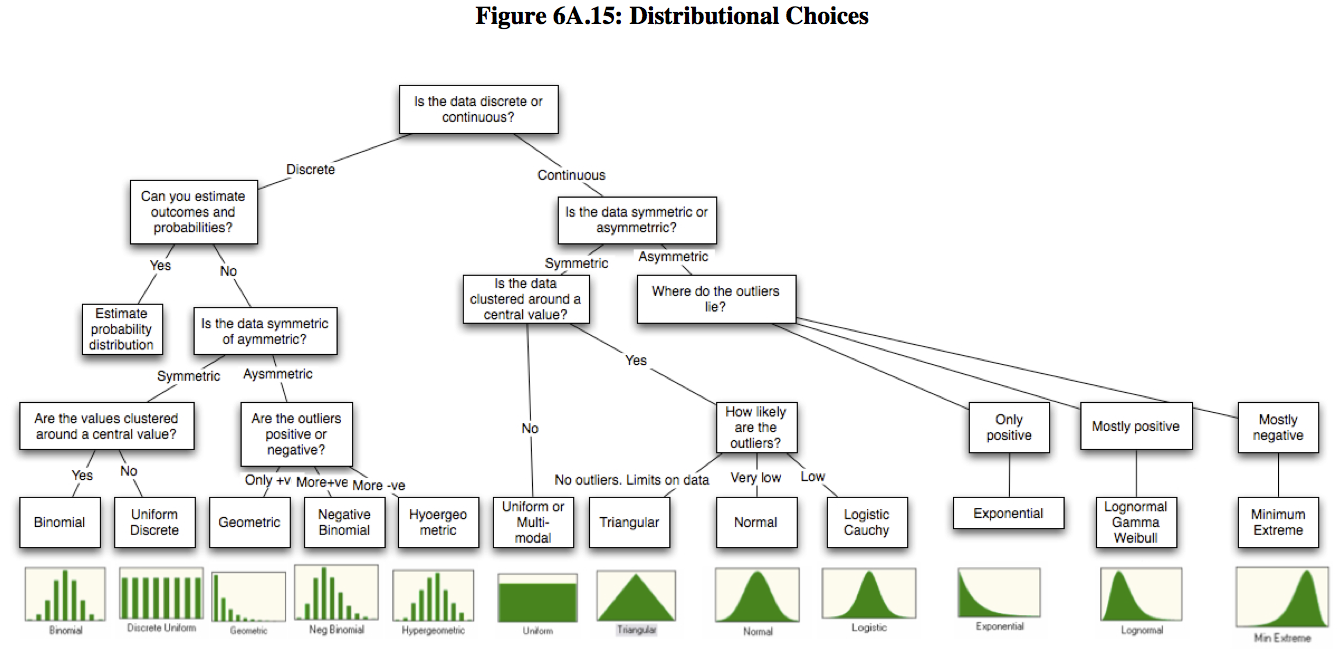
\includegraphics[scale=0.7,bb = 0 0 200 100, draft, type=eps]{distributions.png}\\
Our statistic representing the distance from the predictive request
duration, thus, is continuos 'not only positive and there are no limits
on the data. therefoe, we will choose all the continuos distrubutions
except the Exponential and the Triangular as our hypothesize families
of distributions.


\subsubsection{Estimate parameters:}

After choosing the models that can mathematically represent our data
we have to estimate parameters of such model. There are several estimate
methods in statistical literature, we focused, as we sdudied in statistic
course, on maximum likelihood:\\
We have a random variable with a known pdf f(x,\textgreek{j}) describing
a quantitative character in the population. We should estimate the
vector of costant and unknown parameters \textgreek{j} according to
sampling data: \textbf{$x_{1},x_{2},...,x_{n}$}. \\
Maximum likelihood estimation begins with the mathematical expression
known as a likelihood function of the sample data. Loosely speaking,
the likelihood of a set of data is the probability of obtaining that
particular set of data given the chosen probability model. This expression
contains the unknown parameters. Those values of the parameter that
maximize the sample likelihood are known as the maximum likelihood
estimates (MLE). \\
We define the likelihood function as: $L(x_{1},x_{2},..,x_{n},\vartheta)=\prod_{i=1}^{n}f(x_{i},\vartheta)$
MLE consist in finding \textgreek{j} which maximizes $L(x_{1},x_{2},..,x_{n},\vartheta)$
or its logarithmic function.\\
We can employ mathematical analysis methods (partial derivates equal
to zero) when the likelihood function is rather simple, but very often
we should had using iterative methods. therefore, we implemented using
R method fitdistr() - included in package MASS for maximum-likelihood
fitting of univariate distributions without any information about
likelihood analytical expression. It is enough to specify a data vector,
the type of pdf and eventually the list of starting values for iterative
procedure.


\subsubsection{Goodness of fit tests:}

Goodness of fit tests indicate whether or not it is reasonable to
assume that a random sample comes from a specific distribution. They
are a form of hypothesis testing where the null and alternative hypotheses
are:\\
\\
$H_{0}$: Sample data come from the stated distribution\\
$H_{A}$: Sample data do not come from the stated distribution\\
\\
These tests are sometimes called as omnibus test and they are distribution
free, meaning they do not depend according the pdf.\\
We chose using the Kolmogorov-Smirnov test:\\
This test is used to decide if a sample comes from a population with
a specific distribution.\\
It is restricted to continuous distributions and based on a comparison
between the empirical distribution function (ECDF) and the theoretical
one defined as:\\
$F(x)=\intop_{a}^{x}f(y,\vartheta)dy$ , where f(y,\textgreek{j})
is the pdf.\\
Given n ordered data points $x_{1},x_{2},...x_{n}$ , the ECDF is
defined as:\\
$F_{n}(X_{i})=N(i)/n$ where N(i) is the number of points less than
$X_{i}$($X_{i}$are ordered from smallest to largest value). This
is a step function that increases by 1/n at the value of each ordered
data point.\\
The test statistic used is:\\
$D_{n}=sup_{1\leq i\leq n}|F(X_{i})-F_{n}(X_{i})|$ that is the upper
extreme among absolute value differencies between ECDF and theoretical
CDF.\\
The hypothesis regarding the distributional form is rejected if the
test statistic, $D_{n}$, is greater than the critical value obtained
from a table, or, which is the same, if the p-value is lower than
the significance level.\\
\\
Another test usually taken into consideration is the chi-square goodness
of fit test. But it is applied to binned data, namely data that have
been split into classes. Unfortunately, this test depends consistently
on how the data have been binned.\\
The Kolmogorov-Smirnov test is more powerful than the chi-square test
in the cases in which the sample size is, so to say, unreliable by
the presence of noise, missing values, etc. For large sample sizes
both the tests have the same power. One limitation of the Kolmogorov-Smirnov
test is that the distribution needs to be fully specified. Therefore
the shape and its estimated parameters must be computed beforehand.
That is exactly what our code does.


\subsubsection{R procedure}

The procedure parameters are the data (distances samples) and the
distance of the request duration of a specific features subset event
from the predictive request duration at the anomaly point . The purpose
of the procedure is to select the best shape and the best parameters
for the distributions mentioned above and perform a significance test
of that selection as explained. The goal here cannot be to determine
with certainty what distribution our sample follows. The goal is what
calls parsimonious approximate descriptions of the data. We measure
the P-Value of the given distance according to the distditribution
which explain our data most. and return it for determine if to use
that subset in the next stage. (the procedure is in find\_dist.R)
\end{document}
